\documentclass[fleqn]{rbfin}

%%%%%%%%%%%%%%%%%%%%%%%%%%%%%%%%%%%%
% BEGIN DOCUMENT
%%%%%%%%%%%%%%%%%%%%%%%%%%%%%%%%%%%%
\begin{document}
% Para artigos em PORTUGUÊS, alterar a linha abaixo para \selectlanguage{brazil}
\selectlanguage{english}
\frenchspacing

%%%%%%%%%%%%%%%%%%%%%%%%%%%%%%%%%%%%
% FRONT MATTER
%%%%%%%%%%%%%%%%%%%%%%%%%%%%%%%%%%%%

% ARTICLE TITLE
\title{A Feed-Forward Neural Network for Handwritten Digit Recognition} % Appears on title page

% ARTICLE SHORT TITLE
% \shorttitle{Feed-Forward Neural Network for HDR} % appears on header every other page

% RELEVANT DATES
\nota{Submitted on December 11, 2024.
%
% Revised on May 25, 2024.
% %
% Accepted on June 9, 2024.
% %
% Published online in January 2024.
% %
% Editor in charge: Mr.\ Editor.
}

% AUTHOR INFORMATION
\author{\centering
% Define affiliations
\affiliations{1}{University of Victoria}
\affiliations{2}{ECE 503 Optimization for Machine Learning}
% AUTHOR 1
\textbf{Wang Daming}%
\email{wdm1732418365@gmail.com}
\affiliationlink{1} % Match with the affiliations defined above
% \orcidlink{0000-0000-0000}
\and % separate authors with \and
% % AUTHOR 2
% \textbf{Author Two}%
% \email{author.two@email}
% \affiliationlink{2} % Match with the affiliations defined above
% \orcidlink{0000-0000-0000}
% \and
% % AUTHOR 3
% \textbf{Author Three}%
% \email{author.three@email}
% \affiliationlink{1} % Match with the affiliations defined above
% \affiliationlink{2} % Match with the affiliations defined above
% \orcidlink{0000-0000-0000}
% AND SO ON...
\\[20pt]
% Print the affiliations:
\affiliationname{1}
\affiliationname{2}
}
\autor{Daming Wang, 2024} % appears on header every other page

% JOURNAL INFO
\maketitle
% \pagina{1}
% \rbfd{
% \href
% {http://bibliotecadigital.fgv.br/ojs/index.php/rbfin/index}
% {Revista Brasileira de Finanças (Online)}
% % {Brazilian Review of Finance (Online)},
% Rio de Janeiro,
% \textcolor{BrickRed}{Vol. XX,}
% \textcolor{BrickRed}{No. Y,}
% \textcolor{BrickRed}{August 2024,}
% \textcolor{BrickRed}{pp. x--xx}
% \qquad ISSN 1679-0731, ISSN online 1984-5146}
% \rbfc{\copyright
% 2024
% \href
% {https://www.sbfin.org.br}
% {Sociedade Brasileira de Finanças},
% under a
% \href
% {https://creativecommons.org/licenses/by/4.0/}
% {Creative Commons Attribution 4.0 license} 
% \quad\url{https://doi.org/10.xxxx/xxxxxxxx}
% }
% \rbfe{
% \href
% {http://bibliotecadigital.fgv.br/ojs/index.php/rbfin/index}
% % {Brazilian Review of Finance (Online)}
% {Revista Brasileira de Finanças (Online)}
% XX(Y),
% 2024
% }

% ABSTRACT, KEYWORDS AND JEL
\begin{abstract}
\myabstract{%
% ABSTRACT
This paper shows a small feed-forward neural network for Handwritten Digit Recognition on the MNIST dataset. The code is written in Matlab. I began with the process of loading and preprocessing the data, then convert the digit images into normalized vectors and perform transform class labels into one-hot encodings. The neural network consists of an input layer, a hidden layer, and an output layer. The input layer has 784 input nodes. The hidden layer uses the ReLU activation function, and the output layer uses the softmax function. Together, the model can accuractely predict the digit of the handwritten images from 0 to 9. In order to optimize the model, I use forward and backward passes to compute the loss and gradients to apply mini-batch gradient descent for parameters. The model can achieve a high accuracy on both validation and test sets, which shows the effectiveness of the neural network and the optimization algorithm of our model. The result is shown in the format of a confusion matrix. The complete code is available in the appendix.
}

% KEYWORDS (separated by semicolon)
\keywordslist{MNIST; Neural Network; Handwritten Digit Recognition.}

% JEL CODES (separated by colon)
% \jelcodeslist{E3, C41, C43.}
\end{abstract}

%%%%%%%%%%%%%%%%%%%%%%%%%%%%%%%%%%%%
% END OF FRONT MATTER
%%%%%%%%%%%%%%%%%%%%%%%%%%%%%%%%%%%%

%%%%%%%%%%%%%%%%%%%%%%%%%%%%%%%%%%%%
% DOCUMENT MAIN SECTIONS
%%%%%%%%%%%%%%%%%%%%%%%%%%%%%%%%%%%%
\section{Introduction}\label{sec-intro}

Over the past few years, the field of machine learning met a significant growth especially in the area of deep learning. Moreover, most of the deep learning models are based on neural networks. Since professor metioned how the neural network works in the last few lectures, it made me wonder how we can do with a simple neural networking model and tried to play with it. As for the database, I chose the MNIST since most of the model used to process MNIST dataset is using logistic regression with a fundamental linear model used as a baseline for classification tasks \cite{lecun1998gradient}.



\subsection{Useful tools for reference managing}
There are several useful tools to help organize your references. Here are some of them:
\begin{enumerate}[label=(\roman*), noitemsep]
\item \url{https://www.mendeley.com}
\item \url{https://www.jabref.org}
\item \url{https://www.zotero.org/}
\item \url{https://truben.no/latex/bibtex/}
\end{enumerate}

\section{Methodology}
In this section you should discuss the methodology.\footnote{Footnote links should come after punctuation.}

\subsection{Figures}
Figure~\ref{fig1} was generated in \lstinline/R/ through the following code:
\begin{lstlisting}[language=R]
x = seq(from=0, to=2*pi, length=100)
cm = 1/2.54 # this is just for defining units of measurement
pdf(file='plot.pdf', width=9*cm, height=7*cm, bg=rgb(0,0,0,.1))
par(mai = c(2*cm,1*cm,.5*cm,1*cm))
plot(x, sin(x), type ='l')
dev.off()
\end{lstlisting}

\begin{figure}[ht]
\begin{center}
\caption{A figure}\label{fig1}
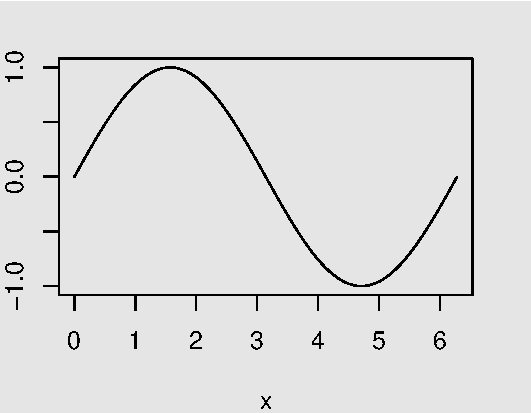
\includegraphics{media/plot.pdf}
\end{center}
\end{figure}

Ideally, the dimensions of the figure should be controlled \emph{outside} of \LaTeX, as the preceding \lstinline/R/ code illustrates. If you cannot generate or obtain the figure with appropriate sizing, then adding the optional argument \lstinline/[width=9cm]/ to the \lstinline/\includegraphics/ command will do the job. Below we illustrate usage of the \lstinline!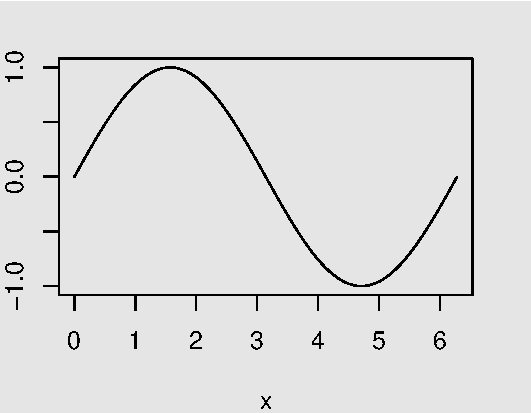
\includegraphics[width=2cm]{media/plot.pdf}! command.

\begin{center}
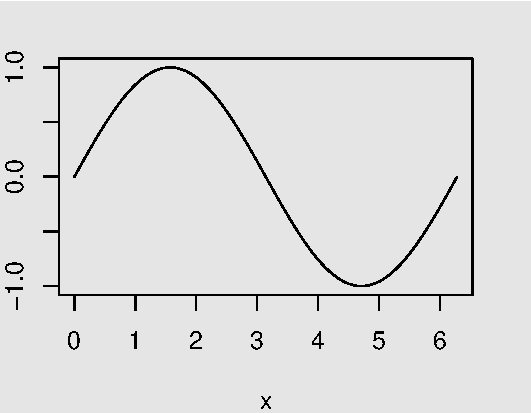
\includegraphics[width=2cm]{media/plot.pdf}
\end{center}

\subsection{The model}

We write inline equations as \(x=x\) or displayed equations as
\begin{equation}\label{eq1}
\mathrm dX_t = \mu\mathrm dt + \sigma\mathrm dB_t
\end{equation}
and reference equations using \lstinline[language=TeX]/\eqref{eq1}/ to display as equation \eqref{eq1}. Maybe we should have added this in \autoref{sec-intro}. You can also reference theorems, for example \lstinline/\autoref{thm:1}/ will produce \autoref{thm:1}.

\begin{definition}
We say that \textbf{$x$ is equal to $x$} whenever $x=x$.
\end{definition}

\begin{lemma}
$x\geq y$ if and only if $y\leq x$.
\end{lemma}
\begin{proof}
This is left as an exercise.
\end{proof}

\begin{proposition}
$x = x$ if and only if $x = x$.
\end{proposition}

\begin{theorem}\label{thm:1}
If $x=x$ and $y=y$, then $x>y$ implies $x>y$.
\end{theorem}

\begin{proof}
A proof with default title.
\end{proof}

\begin{proof}[A proof with custom title]
This is trivial.
\end{proof}

\begin{corollary}
$x>y$ of and only if $y<x$.
\end{corollary}

\begin{remark}
This is a remark.
\end{remark}

\lipsum[2-2]

\section{Results}
You can add tables easily: see \autoref{tab1}. There are three custom column types that accept width specification: \lstinline[]/L/, \lstinline[]/C/ and \lstinline[]/R/, which work similarly to the standard \lstinline[]/p/ column type; for instance, use \lstinline[]/C{4cm}/ for a (horizontally) centered column 4cm wide. Notice, however, that \LaTeX\ has some inconsistencies regarding lengths, as Example \ref{example:lengths} illustrates. Thus, some manual fine-tuning may be necessary to obtain tables with the desired width.

\begin{table}[ht]
\begin{center}
\scalefont{0.9}
\caption{A simple table}\label{tab1}
\begin{tabular}{L{10em}C{5em}c}
\toprule
variable & value & $p$-value\tabularnewline
\midrule
$X$ & 1 & 0.0 \tabularnewline\addlinespace[5pt]
$Y$ & $-1$ & 0.8\tabularnewline
\midrule
{You can write long texts inside\newline table cells, with custom linebreaks} & A & B\tabularnewline
\bottomrule
\end{tabular}
\captionsetup[sub]{width=20em}
\subcaption*{Table descriptions go here. \lipsum[1-1]}
\end{center}
\end{table}



\newpage
\begin{example}\label{example:lengths}
This example illustrates length inconsistencies in \LaTeX.
\begin{table}[ht]
\begin{center}
\rule{.6\textwidth}{1cm}
\begin{tabular}{L{.2\textwidth}C{.2\textwidth}R{.2\textwidth}}
\toprule
a & b & c\tabularnewline\midrule
x & y & z\tabularnewline
\bottomrule
\end{tabular}
\end{center}
\end{table}

The source code yielding the rule and table above is as follows:
\begin{lstlisting}[language = TeX]
\noindent\rule{.6\textwidth}{1cm}
\noindent\begin{tabular}{L{.2\textwidth}C{.2\textwidth}R{.2\textwidth}}
\toprule
x & y & z\tabularnewline\bottomrule
\end{tabular}
\end{lstlisting}
\end{example}

\subsection{Some additional features}
Table~\ref{tab2} illustrates how to align numbers by the decimal place marker. It also shows how to implement the \lstinline[]/\multirow/ command.
\begin{table}[ht]
\begin{center}
\scalefont{0.9}
\caption{Another simple table}\label{tab2}
\begin{tabular}{L{4em}L{4em}r@{.}lc}
\toprule
variable & & \multicolumn{2}{c}{value} & $p$-value\tabularnewline
\midrule
$X$ & & 1&001 & 0.0 \tabularnewline\addlinespace[5pt]
$Y$ & & $-10$&00 & 0.8\tabularnewline\midrule
\multirow{2}{*}{$Z$} & $Z_1$ & 1&1 & 0\tabularnewline
& $Z_2$ & 2&2 & 0\tabularnewline
\bottomrule
\end{tabular}
\end{center}
\end{table}

Here are two useful tools to help formatting \LaTeX\ tables:
\begin{enumerate}[label = (\roman*), itemsep=0pt]
\item \url{https://www.tablesgenerator.com}
\item \url{https://truben.no/table/}
\end{enumerate}
%%%%%%%%%%%%%%%%%%%%%%%%%%%%%%%%%%%%
% END OF DOCUMENT MAIN SECTIONS
%%%%%%%%%%%%%%%%%%%%%%%%%%%%%%%%%%%%


%%%%%%%%%%%%%%%%%%%%%%%%%%%%%%%%%%%%
% ACKNOWLEDGEMENTS
%%%%%%%%%%%%%%%%%%%%%%%%%%%%%%%%%%%%
\paragraph{Acknowledgments}
Author One would like to thank Institution One for financial support.

\paragraph{Conflict of interest} The authors declare no conflict of interest.

\paragraph{Artificial Intelligence} This research utilized AI tools to assist in data analysis, manuscript drafting, and figure generation. All AI-generated content was critically reviewed and validated by the authors to ensure accuracy and alignment with the scientific integrity of the study. The use of AI adhered to ethical guidelines, ensuring transparency and compliance with academic standards. Any biases or limitations inherent to the AI tools were carefully considered in the interpretation of results. The authors affirm that the AI tools did not compromise the originality or integrity of the work.
%%%%%%%%%%%%%%%%%%%%%%%%%%%%%%%%%%%%
% END OF ACKNOWLEDGEMENTS
%%%%%%%%%%%%%%%%%%%%%%%%%%%%%%%%%%%%

%%%%%%%%%%%%%%%%%%%%%%%%%%%%%%%%%%%%
% REFERENCES
%%%%%%%%%%%%%%%%%%%%%%%%%%%%%%%%%%%%
\bibliography{references.bib}\label{refs}
\bibliographystyle{dcu-rbfin}
%%%%%%%%%%%%%%%%%%%%%%%%%%%%%%%%%%%%
% END OF REFERENCES
%%%%%%%%%%%%%%%%%%%%%%%%%%%%%%%%%%%%


%%%%%%%%%%%%%%%%%%%%%%%%%%%%%%%%%%%%

%%%%%%%%%%%%%%%%%%%%%%%%%%%%%%%%%%%%
% APPENDIX
%%%%%%%%%%%%%%%%%%%%%%%%%%%%%%%%%%%%
\rbfinappendix
\section{Matlab Code}

The complete Matlab Code used in this report is listed below: 

loadMNISTImages.m
\begin{lstlisting}
% Load MNIST images from a IDX3-ubyte file
function images = loadMNISTImages(filename)
    % open file with big-endian format
    file = fopen(filename,'r','b');
    % use first 4 bytes to chekc the file type
    if fread(file,1,'int32') ~= 2051
        error('Invalid magic number in %s', filename);
    end
    numImages = fread(file,1,'int32');
    numRows = fread(file,1,'int32');
    numCols = fread(file,1,'int32');
    fprintf('Loading %d images of size %d x %d from %s\n', numImages, numRows, numCols, filename);
    % each pixel is stored as an unsigned byte
    images = fread(file,inf,'unsigned char');
    images = reshape(images, numRows*numCols, numImages);
    images = double(images)/255;
    fclose(file);
    fprintf('Successfully loaded %d images from %s.\n', numImages, filename);
end
\end{lstlisting}

loadMNISTLabels.m

\begin{lstlisting}
% Load MNIST labels from a IDX1-ubyte file
function labels = loadMNISTLabels(filename)
    fid = fopen(filename,'r','b');
    if fread(fid,1,'int32') ~= 2049
        error('Invalid magic number in %s', filename);
    end
    % read the next 4 bytes
    numLabels = fread(fid,1,'int32');
    labels = fread(fid,inf,'unsigned char');
    fclose(fid);
    fprintf('Loading %d labels from %s\n', numLabels, filename);
end
\end{lstlisting}

foward\_pass.m

\begin{lstlisting}
function [Y_hat, cache] = forward_pass(X, W1, b1, W2, b2)
    % X: input
    % 784 * N

    % linear combination for hidden layer neurons
    % 100 * N
    Z1 = W1 * X + b1; 

    % ReLU activation for hidden layer
    A1 = max(Z1, 0);

    % linear combination for output layer neurons
    % 10 * N
    Z2 = W2 * A1 + b2; 

    % softmax function that convert Z2 to probabilities
    exps = exp(Z2 - max(Z2, [], 1));
    Y_hat = exps./sum(exps, 1);

    % store Z1, A1, Z2 for backward_pass function
    cache.Z1 = Z1;
    cache.A1 = A1;
    cache.Z2 = Z2;
end
\end{lstlisting}

backward\_pass.m
\begin{lstlisting}
function [loss, dW1, db1, dW2, db2] = backward_pass(X, Y, W1, b1, W2, b2)
    % get the predicted probabilities and Z1, A1, Z2 from forward_pass
    [Y_hat, cache] = forward_pass(X, W1, b1, W2, b2);
    
    % average the loss and gradients over all samples
    N = size(X,2);

    % compute cross-entropy loss
    loss = -sum(sum(Y .* log(Y_hat+1e-12)))/N;
    
    % gradient of loss of Z2 for output layer
    % 10 * N
    dZ2 = (Y_hat - Y);
    % gradient of W2
    % 10 * 100
    dW2 = (dZ2 * cache.A1')/size(X,2);
    % 10 * 1
    db2 = mean(dZ2,2);
    % 100 * N
    dA1 = W2' * dZ2;
    % ReLU derivative
    dZ1 = dA1 .* (cache.A1>0); 
    % 100 * 784
    dW1 = (dZ1 * X')/size(X,2);
    % 100 * 1
    db1 = mean(dZ1,2);
end

\end{lstlisting}

compute\_loss.m

\begin{lstlisting}
function [loss, acc] = compute_loss(X, Y, W1, b1, W2, b2)
    [Y_hat, ~] = forward_pass(X, W1, b1, W2, b2);
    N = size(X,2);
    loss = -sum(sum(Y.*log(Y_hat+1e-12)))/N;
    [~, pred] = max(Y_hat, [], 1);
    [~, labels] = max(Y, [], 1);
    acc = mean(pred == labels);
end
\end{lstlisting}

project.m
\begin{lstlisting}
    % load training and test data
    train_images = loadMNISTImages('train-images.idx3-ubyte');
    train_labels = loadMNISTLabels('train-labels.idx1-ubyte');
    test_images = loadMNISTImages('t10k-images.idx3-ubyte');
    test_labels = loadMNISTLabels('t10k-labels.idx1-ubyte');
    
    % convert labels to one-hot encoding:
    numClasses = 10;
    Y_train = zeros(numClasses, length(train_labels));
    for i = 1:length(train_labels)
        Y_train(train_labels(i)+1, i) = 1;
    end
    Y_test = zeros(numClasses, length(test_labels));
    for i = 1:length(test_labels)
        Y_test(test_labels(i)+1, i) = 1;
    end
    
    X_train = train_images; % 784 * 60000
    X_test = test_images; % 784 * 10000
    
    % create a validation set from training data to verify the correctness on 
    % training sets to have a basic idea of accuracy.
    val_size = 5000;
    X_val = X_train(:, end-val_size+1:end);
    Y_val = Y_train(:, end-val_size+1:end);
    X_train = X_train(:, 1:end-val_size);
    Y_train = Y_train(:, 1:end-val_size);
    
    % initialize Neural Network Parameters
    % We have 28x28 = 784
    inputSize = 784;
    hiddenSize = 100;
    outputSize = 10;
    
    % make sure the random numbers generated are the same every time
    rng('default');
    % W1 is a matrix of size hiddenSize * inputSize
    % initialize some small random values and scaled by 0.01
    W1 = 0.01*randn(hiddenSize, inputSize);
    b1 = zeros(hiddenSize, 1);
    W2 = 0.01*randn(outputSize, hiddenSize);
    b2 = zeros(outputSize, 1);
    
    % Mini-Batch Gradient Descent Training
    numEpochs = 5;
    batchSize = 128;
    % change the learning_rate
    learning_rate = 0.87;
    fprintf('Learning Rate is %f \n', learning_rate);
    numTrain = size(X_train, 2);
    
    for epoch = 1:numEpochs
        % shuffle training data
        idx = randperm(numTrain);
        X_train = X_train(:, idx);
        Y_train = Y_train(:, idx);
        
        % loop over mini-batches
        for start_i = 1:batchSize:numTrain
            end_i = min(start_i+batchSize-1, numTrain);
            X_batch = X_train(:, start_i:end_i);
            Y_batch = Y_train(:, start_i:end_i);
            [loss, dW1, db1, dW2, db2] = backward_pass(X_batch, Y_batch, W1, b1, W2, b2);
            W1 = W1 - learning_rate * dW1;
            b1 = b1 - learning_rate * db1;
            W2 = W2 - learning_rate * dW2;
            b2 = b2 - learning_rate * db2;
        end
        
        % compute loss on training and validation set
        [train_loss, ~] = compute_loss(X_train, Y_train, W1, b1, W2, b2);
        [val_loss, val_acc] = compute_loss(X_val, Y_val, W1, b1, W2, b2);
        fprintf('Epoch %d: Train Loss = %.4f | Val Loss = %.4f | Val Acc = %.2f%%\n', ...
            epoch, train_loss, val_loss, val_acc*100);
    end
    
    % evaluate on test sets
    [test_loss, test_acc] = compute_loss(X_test, Y_test, W1, b1, W2, b2);
    fprintf('Test Loss = %.4f | Test Accuracy = %.2f%%\n', test_loss, test_acc*100);
    
    % test set confusion matrix
    [Y_hat_test, ~] = forward_pass(X_test, W1, b1, W2, b2);
    [~, pred_test] = max(Y_hat_test, [], 1);
    [~, true_test] = max(Y_test, [], 1);
    confMat = confusionmat(true_test, pred_test);
    disp('Confusion Matrix:');
    disp(confMat);
    
    % normalize the confusion matrix
    confMatNorm = bsxfun(@rdivide, confMat, sum(confMat,2));
    imagesc(confMatNorm);
    colorbar;
    title('Normalized Confusion Matrix');
    xlabel('Predicted Digit');
    ylabel('True Digit');
    axis square;
\end{lstlisting}

Output:

\begin{lstlisting}
Loading 60000 images of size 28 x 28 from train-images.idx3-ubyte
Successfully loaded 60000 images from train-images.idx3-ubyte.
Loading 60000 labels from train-labels.idx1-ubyte
Loading 10000 images of size 28 x 28 from t10k-images.idx3-ubyte
Successfully loaded 10000 images from t10k-images.idx3-ubyte.
Loading 10000 labels from t10k-labels.idx1-ubyte
Learning Rate is 0.870000 
Epoch 1: Train Loss = 0.1412 | Val Loss = 0.1168 | Val Acc = 96.40%
Epoch 2: Train Loss = 0.1053 | Val Loss = 0.0995 | Val Acc = 97.18%
Epoch 3: Train Loss = 0.0941 | Val Loss = 0.0977 | Val Acc = 97.06%
Epoch 4: Train Loss = 0.0567 | Val Loss = 0.0797 | Val Acc = 97.42%
Epoch 5: Train Loss = 0.0577 | Val Loss = 0.0808 | Val Acc = 97.60%
Test Loss = 0.0945 | Test Accuracy = 97.26%
\end{lstlisting}


\mathbb{R} 

% \begin{sidewaystable}
% \begin{center}
% \scalefont{.9}
% \caption{A sideways table}\label{tabA1}
% \begin{tabular}[]{L{6cm}C{2cm}C{2cm}C{2cm}}
% \toprule
% \multirow{2}{*}{variable} & \multicolumn{3}{c}{estimation outputs}\tabularnewline
% \cmidrule(l){2-4}
% & value & $t$-stat. & $p$-value\tabularnewline
% \midrule
% $X$ & 1 & 3.59 & 0.0 \tabularnewline\addlinespace[5pt]
% $Y$ & $-1$ & $-0.1$ & 0.8\tabularnewline
% \midrule
% {You can write long texts inside\newline table cells, with custom linebreaks} & A & B & C\tabularnewline
% \bottomrule
% \end{tabular}
% \end{center}
% \end{sidewaystable}
%%%%%%%%%%%%%%%%%%%%%%%%%%%%%%%%%%%%
% END OF APPENDIX
%%%%%%%%%%%%%%%%%%%%%%%%%%%%%%%%%%%%

\end{document}

%%%%%%%%%%%%%%%%%%%%%%%%%%%%%%%%%%%%
% END OF DOCUMENT
%%%%%%%%%%%%%%%%%%%%%%%%%%%%%%%%%%%%